% 1.2.2
\subsubsection{Thuật toán AES }
\indent Thuật toán AES (Advanced Encryption Standard) là một trong những tiêu chuẩn mã hóa đối xứng được sử dụng rộng rãi nhất hiện nay, được công bố bởi Viện Tiêu chuẩn và Công nghệ Quốc gia Hoa Kỳ (NIST) vào năm 2001, thay thế cho DES (Data Encryption Standard) nhờ hiệu suất cao và độ bảo mật vượt trội. AES được phát triển bởi hai nhà mật mã học người Bỉ, Joan Daemen và Vincent Rijmen, dựa trên thuật toán Rijndael, và được thiết kế để xử lý các khối dữ liệu 128-bit với các độ dài khóa 128, 192, hoặc 256 bit.

\indent AES hoạt động dựa trên một quy trình mã hóa đối xứng, sử dụng cùng một khóa cho cả mã hóa và giải mã, với các vòng lặp (rounds) được thực hiện để tăng cường bảo mật. Các thành phần chính của AES bao gồm:

\begin{itemize}
  \item \textbf{Khóa mã hóa (Encryption Key):} Khóa được sử dụng để mã hóa và giải mã dữ liệu, được mở rộng thông qua thuật toán Key Expansion để tạo ra các khóa vòng (round keys).

  \item \textbf{Trạng thái (State):} Dữ liệu đầu vào (plaintext) được biểu diễn dưới dạng ma trận 4x4 byte, được xử lý qua các bước mã hóa.
\end{itemize}

\indent Hình  ~\ref{fig:cdm4} dưới đây mô tả quy trình mã hóa và giải mã trong thuật toán AES, từ bước chuẩn bị khóa đến quá trình truyền và khôi phục dữ liệu.

\begin{figure}[H]
  \centering
  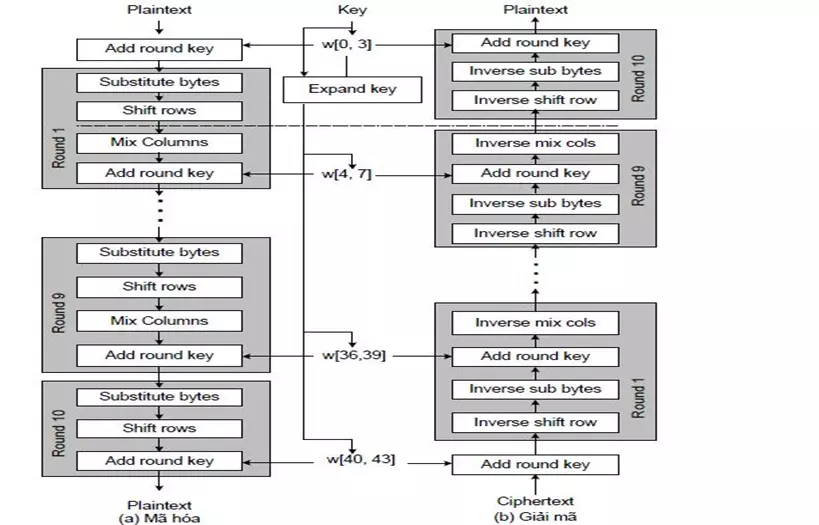
\includegraphics[width=0.95\textwidth]{figures/pic4.png}
  \caption{Quy trình sinh khóa, mã hóa và giải mã trong thuật toán AES.}
  \label{fig:cdm4}
\end{figure}

\indent Hình minh họa ba giai đoạn chính của AES:
\textbf{Giai đoạn 1 – Sinh khóa (Key Expansion): }
    \begin{itemize}
      \item Từ khóa ban đầu, AES sử dụng thuật toán Key Expansion để tạo ra một tập hợp các khóa vòng (round keys) dùng trong từng vòng mã hóa. 
    
      \item Quá trình mở rộng khóa bao gồm các phép:
        \begin{itemize}
          \item \textbf{RotWord:} xoay trái một byte. 
          \item \textbf{SubWord:} thay thế từng byte theo bảng S-box.
          \item \textbf{Rcon:} Xor với Rcon ở vị trí tương ứng và xor với cột cách trước đó 2 cột. 
        \end{itemize}
      \item Kết quả là một chuỗi khóa vòng được sử dụng lần lượt trong các bước AddRoundKey của từng vòng mã hóa.
    \end{itemize}
    
\textbf{Giai đoạn 2 – Mã hóa (Encryption):} 
    \begin{itemize}
      \item Quá trình mã hóa trong AES biến đổi dữ liệu đầu vào (plaintext) thành bản mã (ciphertext) thông qua nhiều vòng lặp, mỗi vòng gồm các phép biến đổi tuyến tính và phi tuyến nhằm khuếch tán và xáo trộn thông tin.
    
      \item Hình ~\ref{fig:cdm5} dưới đây mô tả quy trình mã hóa trong thuật toán AES, từ bước mở rộng khóa đến quá trình thực hiện các vòng mã hóa để tạo ra bản mã (ciphertext).
      
        \begin{figure}[H]
          \centering
          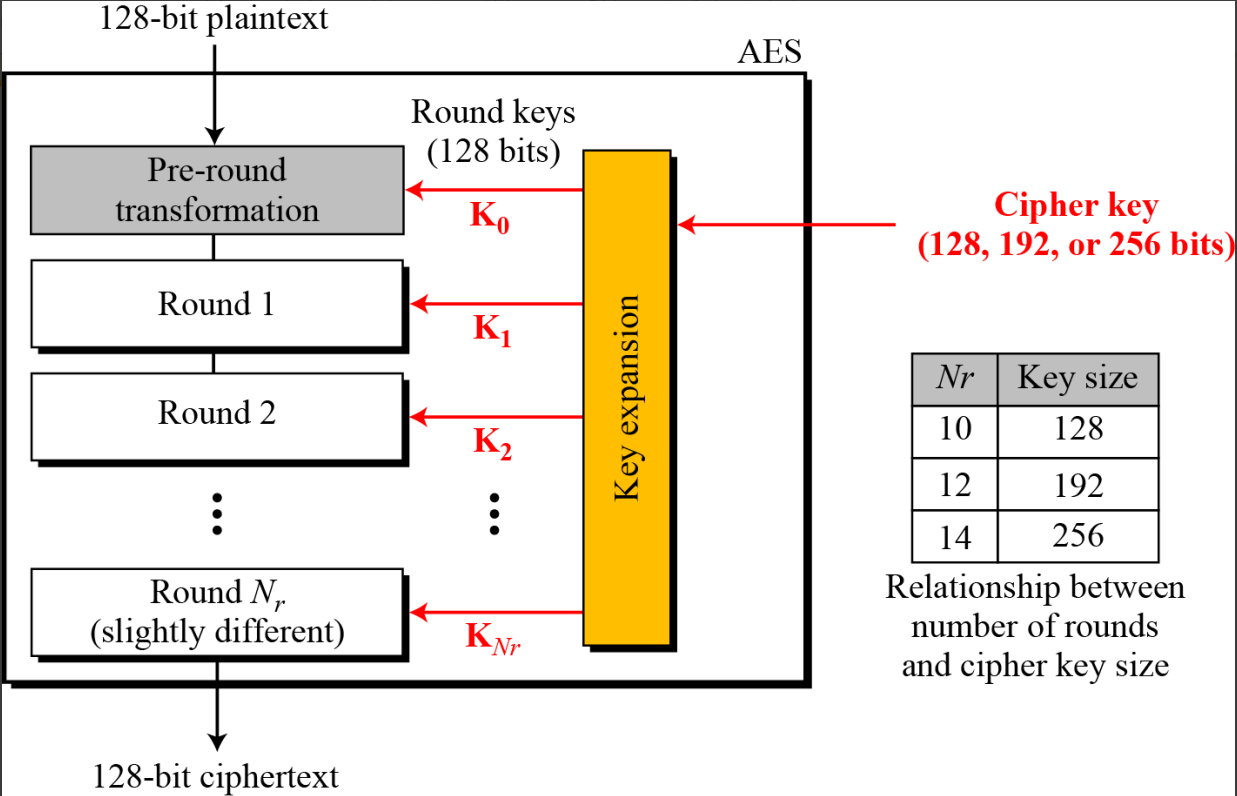
\includegraphics[width=0.85\textwidth]{figures/pic5.png}
          \caption{Quy trình mã hóa AES tổng quát.}
          \label{fig:cdm5}
        \end{figure}
        
      \item Từ sơ đồ quy trình mã hóa tổng quát có thể thấy, mỗi vòng mã hóa trong AES thực hiện một chuỗi phép biến đổi dữ liệu. Hình ~\ref{fig:cdm6} dưới đây mô tả chi tiết cấu trúc của một vòng mã hóa.
      
        \begin{figure}[H]
          \centering
          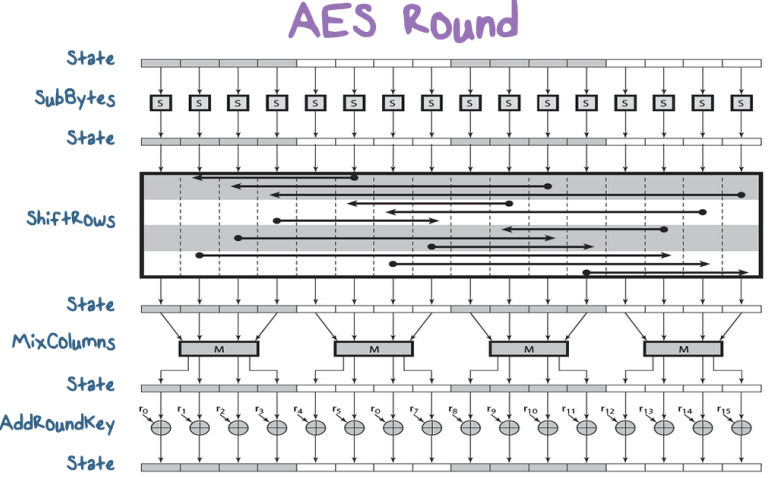
\includegraphics[width=.85\textwidth]{figures/pic6.png}
          \caption{Cấu trúc một vòng mã hóa AES.}
          \label{fig:cdm6}
        \end{figure}

      \item Gồm bốn phép biến đổi chính:

        \begin{itemize}
          \item \textbf{SubBytes:} Thay thế từng byte trong ma trận State bằng giá trị tương ứng trong bảng S-box để tạo tính phi tuyến.
          \item \textbf{ShiftRows:} Dịch vòng các hàng trong ma trận State, giúp khuếch tán dữ liệu theo hàng.
          \item \textbf{MixColumns:} Trộn các byte trong từng cột bằng phép nhân ma trận trong trường hữu hạn GF(2⁸), tăng độ khuếch tán (bỏ qua trong vòng cuối).
          \item \textbf{AddRoundKey:} Mỗi byte của State được XOR với byte tương ứng trong khóa vòng.
        \end{itemize}
      \item Một chuỗi khóa vòng được sử dụng lần lượt trong các bước AddRoundKey của từng vòng mã hóa.
    \end{itemize}
\textbf{Giai đoạn 3 – Giải mã (Decryption):} 
    \begin{itemize}
      \item Quá trình giải mã trong AES thực hiện ngược lại quy trình mã hóa, sử dụng cùng khóa bí mật.
    
      \item Các phép biến đổi được đảo ngược theo thứ tự:
        \begin{itemize}
          \item \textbf{AddRoundKey:} XOR dữ liệu với khóa vòng tương ứng.
          \item \textbf{InvMixColumns:} trộn cột theo phép nghịch đảo trong trường GF(2⁸) (bỏ qua trong vòng cuối).
          \item \textbf{InvShiftRows:} dịch các hàng theo chiều ngược lại so với mã hóa.
          \item \textbf{InvSubBytes:} thay thế các byte bằng giá trị trong bảng nghịch đảo S-box.
        \end{itemize}
      \item Kết quả thu được là bản rõ (plaintext) ban đầu.
    \end{itemize}
  

\indent Quy trình này đảm bảo độ an toàn của AES nhờ vào sự phức tạp của các phép toán ma trận và sự phụ thuộc vào khóa, làm cho việc giải mã mà không có khóa trở nên cực kỳ khó khăn, ngay cả với các phương pháp tấn công brute-force. Trong hệ thống nhắn tin bảo mật, AES được sử dụng để mã hóa nội dung tin nhắn, kết hợp với RSA để bảo vệ khóa AES trong quá trình trao đổi, như được mô tả trong CIST 140 (Section 3.2, 3.4), tạo ra một lớp bảo mật mạnh mẽ chống lại các mối đe dọa như nghe lén và sửa đổi dữ liệu.
